\documentclass{beamer}
\usepackage{tikz}

\usetheme{metropolis}           % Use metropolis theme

\usepackage{helvet}
\renewcommand{\familydefault}{\sfdefault}


\title{Securing IoT Networks through Moving Target Defence}
\subtitle{Advanced Cybersecurity}

\date{Jun 23, 2025}
\author{%
  Andrei Vlădescu\inst{1} \and
  Prof. dr. ing. Ion Bica\inst{2}
}
\addtobeamertemplate{title page}{
  \begin{tikzpicture}[remember picture,overlay]
    \node[anchor=north east, xshift=0.1cm, yshift=-6.9cm]
      at (current page.north east)
      {
\includegraphics[height=2.5cm]{images/logo/upb.png}};
  \end{tikzpicture}
}{}

\institute[UNSTPB]{
  \inst{1} University Politehnica of Bucharest (UPB)\\
  \inst{2} “Ferdinand I” Military Technical Academy
}

\begin{document}

\maketitle


% 1. Introduction
\section{Introduction}

\begin{frame}{Context \& Motivation}
  \begin{itemize}
    \item Explosion of IoT devices in smart homes, healthcare, critical infrastructure
    \item Resource constraints \& lack of built-in security 
    \item IoT as attractive targets for large-scale DDoS attacks
  \end{itemize}
\end{frame}

\begin{frame}{Research Objectives}
  \begin{itemize}
    \item Evaluate Moving Target Defence (MTD) for IoT security
    \item Integrate MTD with Software-Defined Networking (SDN)
    \item Evaluate the solution in a public network
  \end{itemize}

  \note{}
\end{frame}

\begin{frame}{State-of-the-Art \& Where We Fit}
\begin{itemize}
    \item \textbf{Mutable Networks (MUTE)} – crypto-shuffled IP/port mapping
    \item \textbf{Random Host Mutation (RHM)} – edge IP shuffling
    \item \textbf{OF-RHM (OpenFlow)} – SDN-based randomization
  \end{itemize}
\end{frame}

% 2. Proposed Architecture
\section{Proposed Architecture}

\begin{frame}{Threat Model}
  \begin{itemize}
    \item Botnet-driven volumetric DDoS (SYN/UDP flooding)  
    \item Target: resource-constrained IoT devices (no IDS/ACL)
  \end{itemize}
\end{frame}

\begin{frame}{System Architecture}
  \begin{center}
    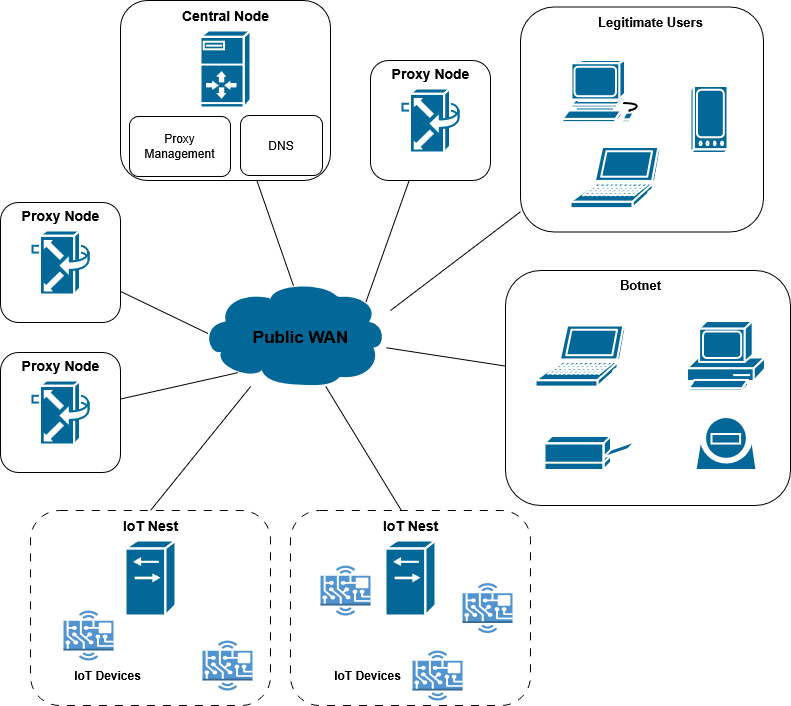
\includegraphics[width=0.83\textwidth]{presentation/images/system_architecture.png}
  \end{center}
  
\end{frame}

\begin{frame}{Defence Workflow}
  \begin{center}
    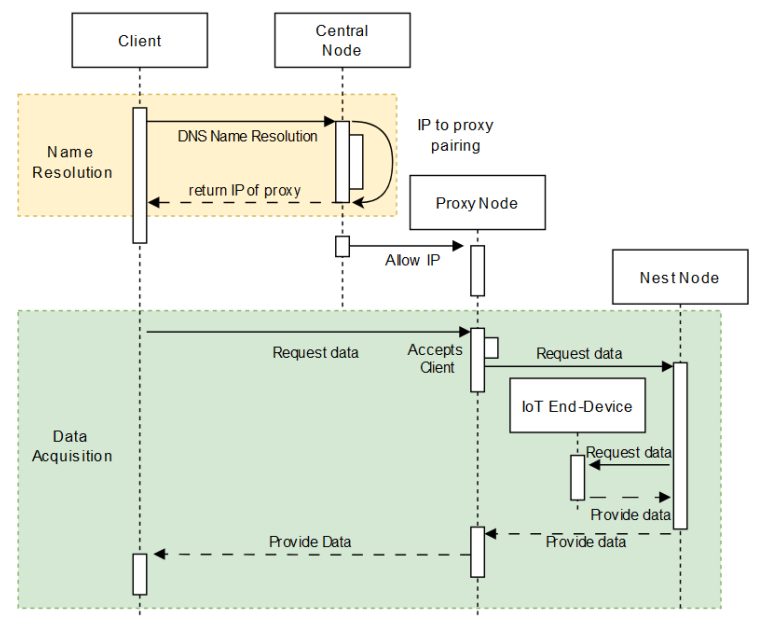
\includegraphics[width=0.83\textwidth]{presentation/images/sequence_diagram.png}
  \end{center}
\end{frame}

% 3. Results & Insights
\section{Results \& Insights}

\begin{frame}{Simulation Environment}
    Ixia Breakingpoint Data Rate Curve
    \vspace{1em}
    \begin{center}
        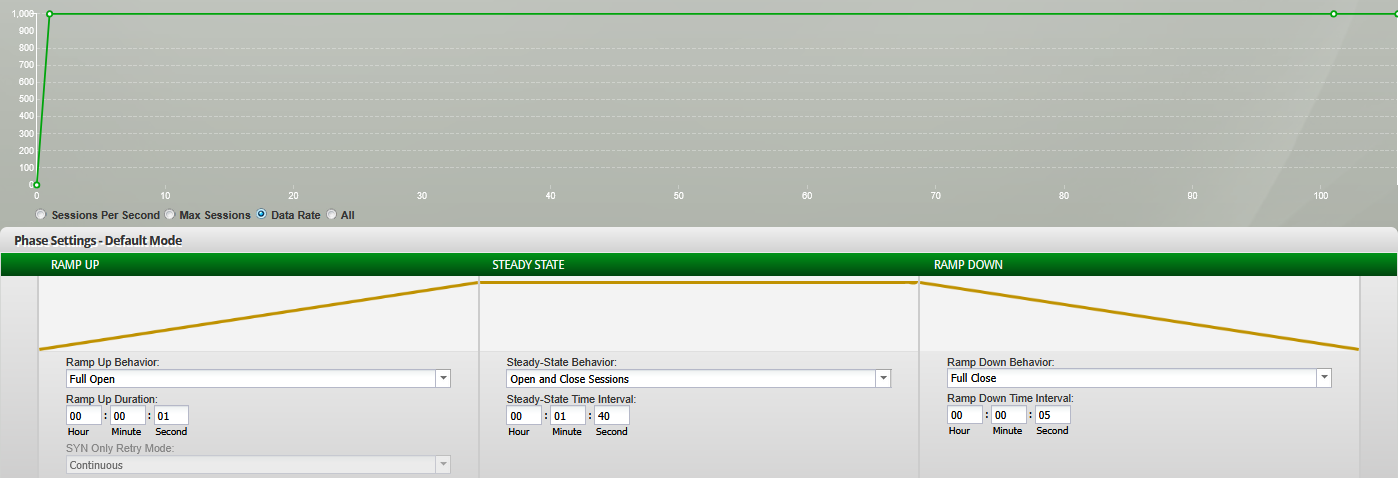
\includegraphics[width=\textwidth]{images/breakingpoint_curve.png}
    \end{center}
\end{frame}

\begin{frame}{Statistics}
    Nominal Usage
    \vspace{1em}
    \begin{center}
        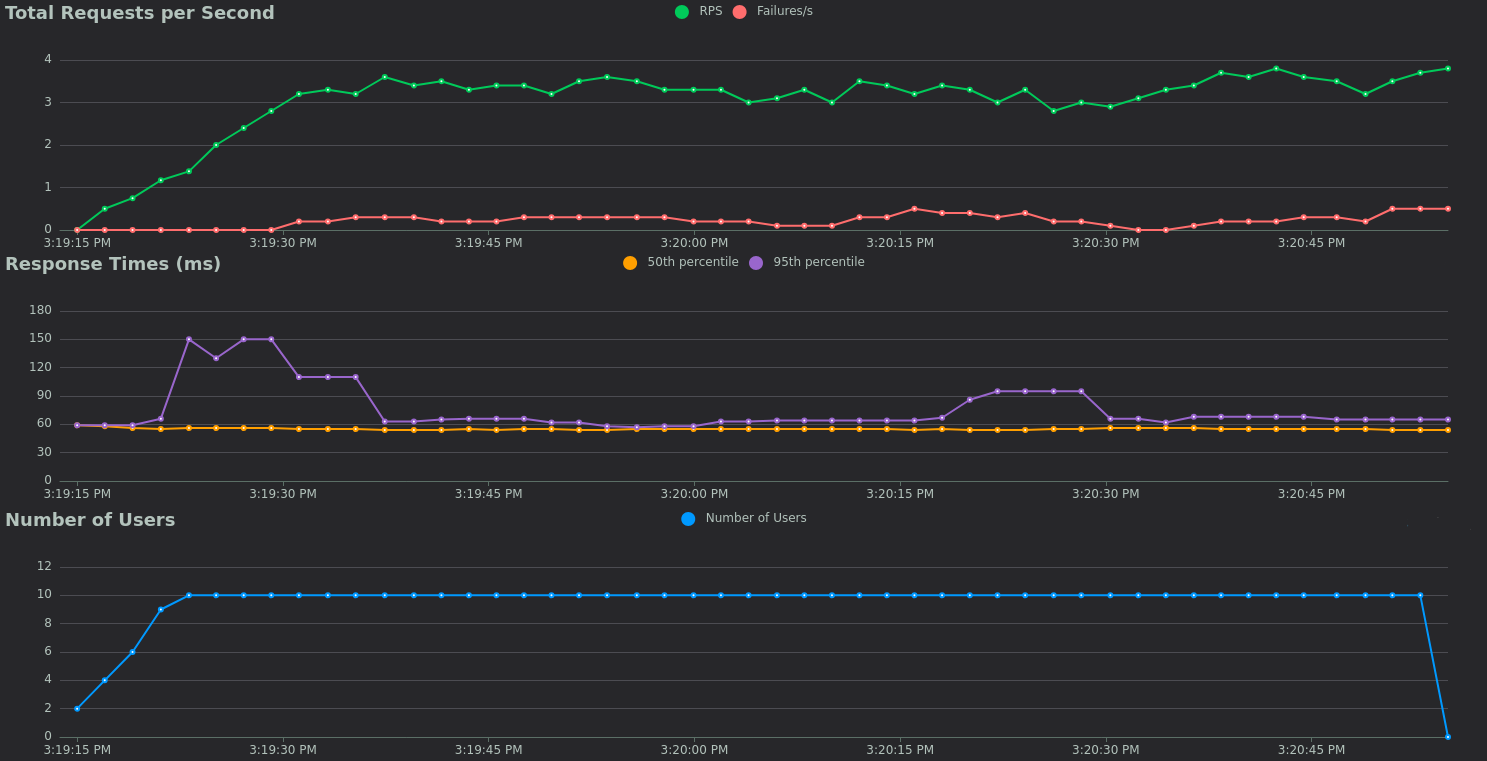
\includegraphics[width=\textwidth]{images/nominal_usage.png}
    \end{center}
\end{frame}

\begin{frame}{Statistics}
    Unprotected Attack
    \vspace{1em}
    \begin{center}
        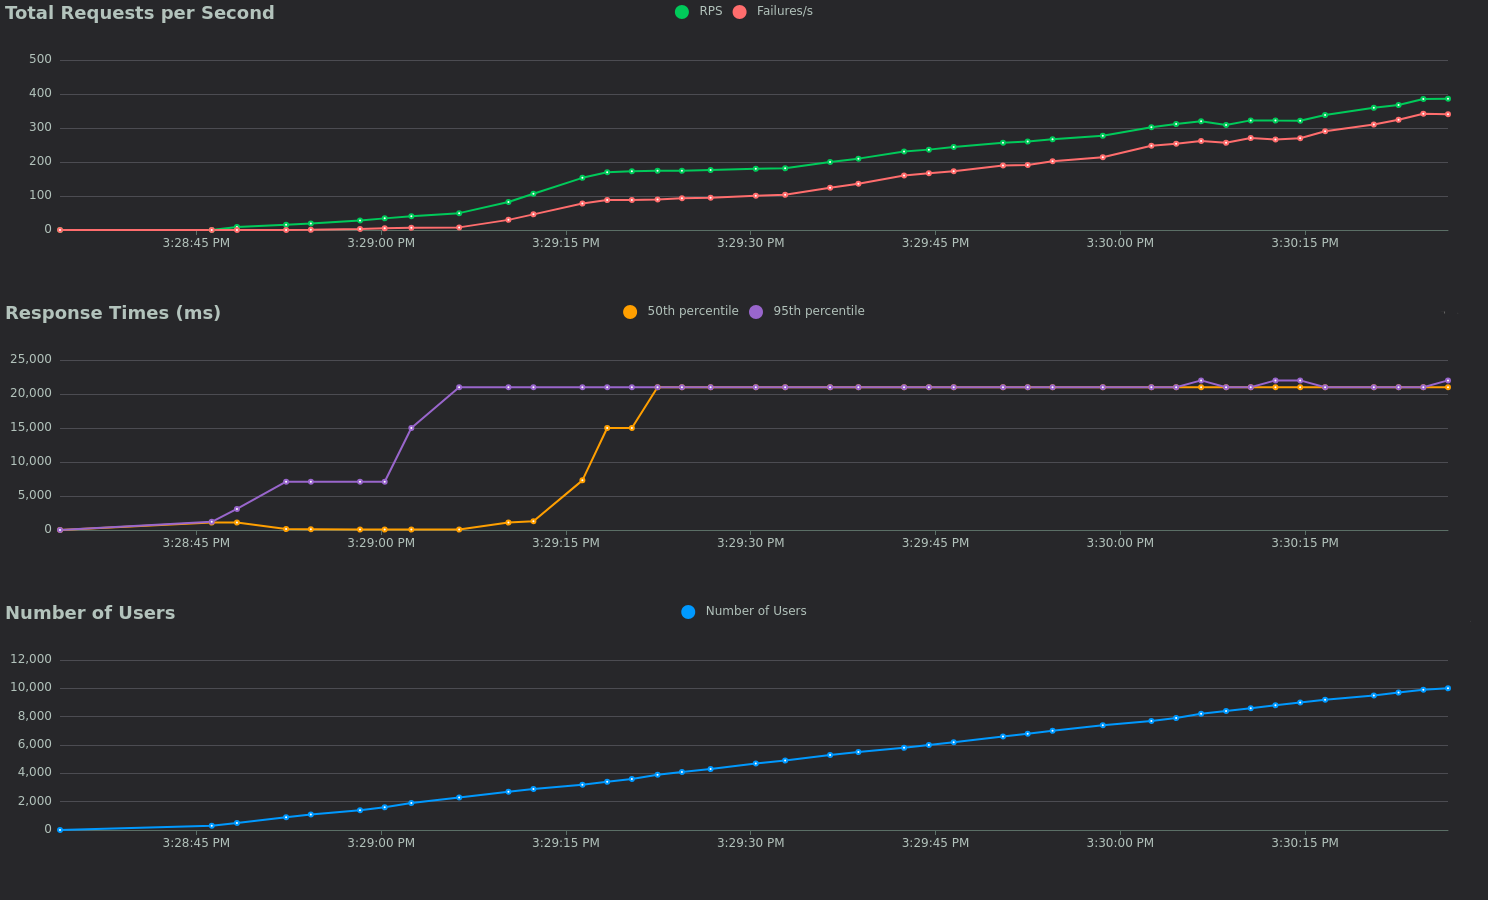
\includegraphics[width=\textwidth]{images/ddos_usage.png}
    \end{center}
\end{frame}

\begin{frame}{Statistics}
Power Draw
    \vspace{1em}

  \begin{center}
    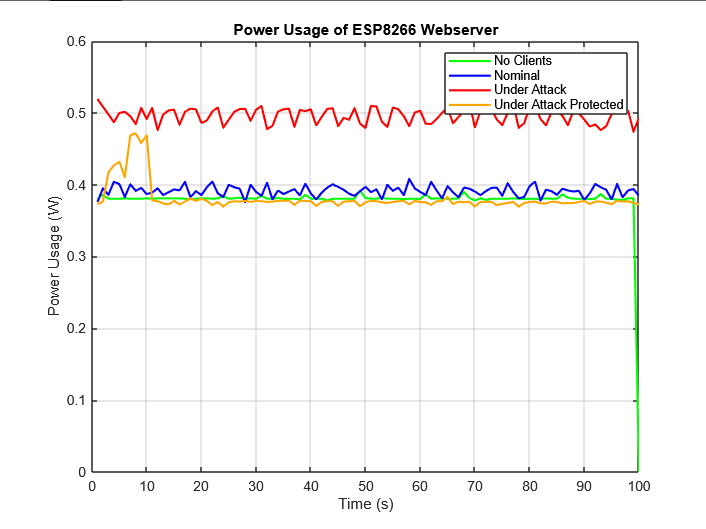
\includegraphics[width=0.8\textwidth]{images/power_usage_esp8266.png}
  \end{center}
\end{frame}

% Q&A
\begin{frame}{Q\&A}
  \centering Thank you!\par
  \vspace{1em}
  \large Any questions?
\end{frame}

\end{document}
